\section{Drawing Functions}

Drawing functions work with matrices/images of arbitrary depth.
The boundaries of the shapes can be rendered with antialiasing (implemented only for 8-bit images for now).
All the functions include the parameter color that uses a rgb value (that may be constructed
with \texttt{CV\_RGB} \cvC{macro or the \cvCppCross{cvScalar} function}
\cvCpp{or the \cross{Scalar} constructor}) for color
images and brightness for grayscale images. For color images the order channel
is normally \emph{Blue, Green, Red}, this is what \cvCppCross{imshow}, \cvCppCross{imread} and \cvCppCross{imwrite} expect
\ifCpp
, so if you form a color using \cross{Scalar} constructor, it should look like:
\[\texttt{Scalar}(blue\_component, green\_component, red\_component[, alpha\_component])\]
\fi
\ifC
, so if you form a color using \cvCppCross{cvScalar}, it should look like:
\[\texttt{cvScalar}(blue\_component, green\_component, red\_component[, alpha\_component])\]
\fi

If you are using your own image rendering and I/O functions, you can use any channel ordering, the drawing functions process each channel independently and do not depend on the channel order or even on the color space used. The whole image can be converted from BGR to RGB or to a different color space using \cvCppCross{cvtColor}.

If a drawn figure is partially or completely outside the image, the drawing functions clip it. Also, many drawing functions can handle pixel coordinates specified with sub-pixel accuracy, that is, the coordinates can be passed as fixed-point numbers, encoded as integers. The number of fractional bits is specified by the \texttt{shift} parameter and the real point coordinates are calculated as $\texttt{Point}(x,y)\rightarrow\texttt{Point2f}(x*2^{-shift},y*2^{-shift})$. This feature is especially effective wehn rendering antialiased shapes.

Also, note that the functions do not support alpha-transparency - when the target image is 4-channnel, then the \texttt{color[3]} is simply copied to the repainted pixels. Thus, if you want to paint semi-transparent shapes, you can paint them in a separate buffer and then blend it with the main image.

\ifCPy

\cvCPyFunc{Circle}
Draws a circle.

\cvdefC{void cvCircle( \par CvArr* img,\par CvPoint center,\par int radius,\par CvScalar color,\par int thickness=1,\par int lineType=8,\par int shift=0 );}
\cvdefPy{Circle(img,center,radius,color,thickness=1,lineType=8,shift=0)-> None}

\begin{description}
\cvarg{img}{Image where the circle is drawn}
\cvarg{center}{Center of the circle}
\cvarg{radius}{Radius of the circle}
\cvarg{color}{Circle color}
\cvarg{thickness}{Thickness of the circle outline if positive, otherwise this indicates that a filled circle is to be drawn}
\cvarg{lineType}{Type of the circle boundary, see \cross{Line} description}
\cvarg{shift}{Number of fractional bits in the center coordinates and radius value}
\end{description}

The function draws a simple or filled circle with a
given center and radius.

\cvCPyFunc{ClipLine}
Clips the line against the image rectangle.

\cvdefC{int cvClipLine( \par CvSize imgSize,\par CvPoint* pt1,\par CvPoint* pt2 );}
\cvdefPy{ClipLine(imgSize, pt1, pt2) -> (clipped\_pt1, clipped\_pt2)}
\begin{description}
\cvarg{imgSize}{Size of the image}
\cvarg{pt1}{First ending point of the line segment. \cvC{It is modified by the function.}}
\cvarg{pt2}{Second ending point of the line segment. \cvC{It is modified by the function.}}
\end{description}

The function calculates a part of the line segment which is entirely within the image.
\cvC{It returns 0 if the line segment is completely outside the image and 1 otherwise.}
\cvPy{If the line segment is outside the image, it returns None. If the line segment is inside the image it returns a new pair of points.}

\cvCPyFunc{DrawContours}
Draws contour outlines or interiors in an image.

\cvdefC{
void cvDrawContours( \par CvArr *img,\par CvSeq* contour,\par CvScalar external\_color,\par CvScalar hole\_color,\par int max\_level,\par int thickness=1,\par int lineType=8 );
}
\cvdefPy{DrawContours(img,contour,external\_color,hole\_color,max\_level,thickness=1,lineType=8,offset=(0,0))-> None}

\begin{description}
\cvarg{img}{Image where the contours are to be drawn. As with any other drawing function, the contours are clipped with the ROI.}
\cvarg{contour}{Pointer to the first contour}
\cvarg{external\_color}{Color of the external contours}
\cvarg{hole\_color}{Color of internal contours (holes)}
\cvarg{max\_level}{Maximal level for drawn contours. If 0, only
\texttt{contour} is drawn. If 1, the contour and all contours following
it on the same level are drawn. If 2, all contours following and all
contours one level below the contours are drawn, and so forth. If the value
is negative, the function does not draw the contours following after
\texttt{contour} but draws the child contours of \texttt{contour} up
to the $|\texttt{max\_level}|-1$ level.}
\cvarg{thickness}{Thickness of lines the contours are drawn with.
If it is negative (For example, =CV\_FILLED), the contour interiors are
drawn.}
\cvarg{lineType}{Type of the contour segments, see \cross{Line} description}
\end{description}

The function draws contour outlines in the image if $\texttt{thickness} \ge 0$ or fills the area bounded by the contours if $ \texttt{thickness}<0$.

\ifC
Example: Connected component detection via contour functions

\begin{lstlisting}
#include "cv.h"
#include "highgui.h"

int main( int argc, char** argv )
{
    IplImage* src;
    // the first command line parameter must be file name of binary 
    // (black-n-white) image
    if( argc == 2 && (src=cvLoadImage(argv[1], 0))!= 0)
    {
        IplImage* dst = cvCreateImage( cvGetSize(src), 8, 3 );
        CvMemStorage* storage = cvCreateMemStorage(0);
        CvSeq* contour = 0;

        cvThreshold( src, src, 1, 255, CV_THRESH_BINARY );
        cvNamedWindow( "Source", 1 );
        cvShowImage( "Source", src );

        cvFindContours( src, storage, &contour, sizeof(CvContour), 
           CV_RETR_CCOMP, CV_CHAIN_APPROX_SIMPLE );
        cvZero( dst );

        for( ; contour != 0; contour = contour->h_next )
        {
            CvScalar color = CV_RGB( rand()&255, rand()&255, rand()&255 );
            /* replace CV_FILLED with 1 to see the outlines */
            cvDrawContours( dst, contour, color, color, -1, CV_FILLED, 8 );
        }

        cvNamedWindow( "Components", 1 );
        cvShowImage( "Components", dst );
        cvWaitKey(0);
    }
}
\end{lstlisting}
\fi

\cvCPyFunc{Ellipse}
Draws a simple or thick elliptic arc or an fills ellipse sector.

\cvdefC{void cvEllipse( \par CvArr* img,\par CvPoint center,\par CvSize axes,\par double angle,\par double start\_angle,\par double end\_angle,\par CvScalar color,\par int thickness=1,\par int lineType=8,\par int shift=0 );}
\cvdefPy{Ellipse(img,center,axes,angle,start\_angle,end\_angle,color,thickness=1,lineType=8,shift=0)-> None}

\begin{description}
\cvarg{img}{The image}
\cvarg{center}{Center of the ellipse}
\cvarg{axes}{Length of the ellipse axes}
\cvarg{angle}{Rotation angle}
\cvarg{start\_angle}{Starting angle of the elliptic arc}
\cvarg{end\_angle}{Ending angle of the elliptic arc.}
\cvarg{color}{Ellipse color}
\cvarg{thickness}{Thickness of the ellipse arc outline if positive, otherwise this indicates that a filled ellipse sector is to be drawn}
\cvarg{lineType}{Type of the ellipse boundary, see \cross{Line} description}
\cvarg{shift}{Number of fractional bits in the center coordinates and axes' values}
\end{description}

The function draws a simple or thick elliptic
arc or fills an ellipse sector. The arc is clipped by the ROI rectangle.
A piecewise-linear approximation is used for antialiased arcs and
thick arcs. All the angles are given in degrees. The picture below
explains the meaning of the parameters.

Parameters of Elliptic Arc

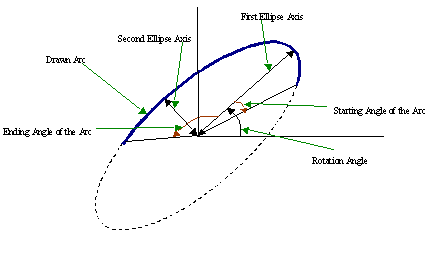
\includegraphics[width=0.5\textwidth]{pics/ellipse.png}

\cvCPyFunc{EllipseBox}

Draws a simple or thick elliptic arc or fills an ellipse sector.

\cvdefC{void cvEllipseBox( \par CvArr* img, \par CvBox2D box, \par CvScalar color,
                   \par int thickness=1, \par int lineType=8, \par int shift=0 );}
\cvdefPy{EllipseBox(img,box,color,thickness=1,lineType=8,shift=0)-> None}

\begin{description}
\cvarg{img}{Image}
\cvarg{box}{The enclosing box of the ellipse drawn}
\cvarg{thickness}{Thickness of the ellipse boundary}
\cvarg{lineType}{Type of the ellipse boundary, see \cross{Line} description}
\cvarg{shift}{Number of fractional bits in the box vertex coordinates}
\end{description}

The function draws a simple or thick ellipse outline, or fills an ellipse. The functions provides a convenient way to draw an ellipse approximating some shape; that is what \cross{CamShift} and \cross{FitEllipse} do. The ellipse drawn is clipped by ROI rectangle. A piecewise-linear approximation is used for antialiased arcs and thick arcs.

\cvCPyFunc{FillConvexPoly}
Fills a convex polygon.

\cvdefC{
void cvFillConvexPoly( \par CvArr* img,\par CvPoint* pts,\par int npts,\par CvScalar color,\par int lineType=8,\par int shift=0 );}
\cvdefPy{FillConvexPoly(img,pn,color,lineType=8,shift=0)-> None}

\begin{description}
\cvarg{img}{Image}
\ifC
\cvarg{pts}{Array of pointers to a single polygon}
\cvarg{npts}{Polygon vertex counter}
\else
\cvarg{pn}{List of coordinate pairs}
\fi
\cvarg{color}{Polygon color}
\cvarg{lineType}{Type of the polygon boundaries, see \cross{Line} description}
\cvarg{shift}{Number of fractional bits in the vertex coordinates}
\end{description}

The function fills a convex polygon's interior.
This function is much faster than the function \texttt{cvFillPoly}
and can fill not only convex polygons but any monotonic polygon,
i.e., a polygon whose contour intersects every horizontal line (scan
line) twice at the most.


\cvCPyFunc{FillPoly}
Fills a polygon's interior.

\cvdefC{
void cvFillPoly( \par CvArr* img,\par CvPoint** pts,\par int* npts,\par int contours,\par CvScalar color,\par int lineType=8,\par int shift=0 );
}
\cvdefPy{FillPoly(img,polys,color,lineType=8,shift=0)-> None}

\begin{description}
\cvarg{img}{Image}
\ifC
\cvarg{pts}{Array of pointers to polygons}
\cvarg{npts}{Array of polygon vertex counters}
\cvarg{contours}{Number of contours that bind the filled region}
\fi
\ifPy
\cvarg{polys}{List of lists of (x,y) pairs.  Each list of points is a polygon.}
\fi
\cvarg{color}{Polygon color}
\cvarg{lineType}{Type of the polygon boundaries, see \cross{Line} description}
\cvarg{shift}{Number of fractional bits in the vertex coordinates}
\end{description}


The function fills an area bounded by several
polygonal contours. The function fills complex areas, for example,
areas with holes, contour self-intersection, and so forth.

\cvCPyFunc{GetTextSize}
Retrieves the width and height of a text string.

\cvdefC{
void cvGetTextSize( \par const char* textString,\par const CvFont* font,\par CvSize* textSize,\par int* baseline );}
\cvdefPy{GetTextSize(textString,font)-> (textSize,baseline)}

\begin{description}
\cvarg{font}{Pointer to the font structure}
\cvarg{textString}{Input string}
\cvarg{textSize}{Resultant size of the text string. Height of the text does not include the height of character parts that are below the baseline.}
\cvarg{baseline}{y-coordinate of the baseline relative to the bottom-most text point}
\end{description}

The function calculates the dimensions of a rectangle to enclose a text string when a specified font is used.

\cvCPyFunc{InitFont}
Initializes font structure.

\cvdefC{
void cvInitFont( \par CvFont* font,\par int fontFace,\par double hscale,\par double vscale,\par double shear=0,\par int thickness=1,\par int lineType=8 );}
\cvdefPy{InitFont(fontFace,hscale,vscale,shear=0,thickness=1,lineType=8)-> font}

\begin{description}
\cvarg{font}{Pointer to the font structure initialized by the function}
\cvarg{fontFace}{Font name identifier. Only a subset of Hershey fonts \url{http://sources.isc.org/utils/misc/hershey-font.txt} are supported now:
 \begin{description}
 \cvarg{CV\_FONT\_HERSHEY\_SIMPLEX}{normal size sans-serif font}
 \cvarg{CV\_FONT\_HERSHEY\_PLAIN}{small size sans-serif font}
 \cvarg{CV\_FONT\_HERSHEY\_DUPLEX}{normal size sans-serif font (more complex than \par \texttt{CV\_FONT\_HERSHEY\_SIMPLEX})}
 \cvarg{CV\_FONT\_HERSHEY\_COMPLEX}{normal size serif font}
 \cvarg{CV\_FONT\_HERSHEY\_TRIPLEX}{normal size serif font (more complex than \texttt{CV\_FONT\_HERSHEY\_COMPLEX})}
 \cvarg{CV\_FONT\_HERSHEY\_COMPLEX\_SMALL}{smaller version of \texttt{CV\_FONT\_HERSHEY\_COMPLEX}}
 \cvarg{CV\_FONT\_HERSHEY\_SCRIPT\_SIMPLEX}{hand-writing style font}
 \cvarg{CV\_FONT\_HERSHEY\_SCRIPT\_COMPLEX}{more complex variant of \texttt{CV\_FONT\_HERSHEY\_SCRIPT\_SIMPLEX}}
 \end{description}
 The parameter can be composited from one of the values above and an optional \texttt{CV\_FONT\_ITALIC} flag, which indicates italic or oblique font.}
\cvarg{hscale}{Horizontal scale.  If equal to \texttt{1.0f}, the characters have the original width depending on the font type. If equal to \texttt{0.5f}, the characters are of half the original width.}
\cvarg{vscale}{Vertical scale. If equal to \texttt{1.0f}, the characters have the original height depending on the font type. If equal to \texttt{0.5f}, the characters are of half the original height.}
\cvarg{shear}{Approximate tangent of the character slope relative to the vertical line.  A zero value means a non-italic font, \texttt{1.0f} means about a 45 degree slope, etc.} 
\cvarg{thickness}{Thickness of the text strokes}
\cvarg{lineType}{Type of the strokes, see \cross{Line} description}
\end{description}

The function initializes the font structure that can be passed to text rendering functions.


\cvCPyFunc{InitLineIterator}
Initializes the line iterator.

\cvdefC{
int cvInitLineIterator( \par const CvArr* image,\par CvPoint pt1,\par CvPoint pt2,\par CvLineIterator* line\_iterator,\par int connectivity=8,\par int left\_to\_right=0 );
}
\cvdefPy{InitLineIterator(image, pt1, pt2, connectivity=8, left\_to\_right=0) -> line\_iterator}

\begin{description}
\cvarg{image}{Image to sample the line from}
\cvarg{pt1}{First ending point of the line segment}
\cvarg{pt2}{Second ending point of the line segment}
\cvC{\cvarg{line\_iterator}{Pointer to the line iterator state structure}}
\cvarg{connectivity}{The scanned line connectivity, 4 or 8.}
\cvarg{left\_to\_right}{
If ($ \texttt{left\_to\_right} = 0 $ ) then the line is scanned in the specified order, from \texttt{pt1} to \texttt{pt2}.
If ($ \texttt{left\_to\_right} \ne 0$) the line is scanned from left-most point to right-most.}
\cvPy{\cvarg{line\_iterator}{Iterator over the pixels of the line}}
\end{description}

\ifC
The function initializes the line
iterator and returns the number of pixels between the two end points.
Both points must be inside the image.
After the iterator has been
initialized, all the points on the raster line that connects the
two ending points may be retrieved by successive calls of
\texttt{CV\_NEXT\_LINE\_POINT} point.
\fi
\ifPy
The function returns an iterator over the pixels connecting the two points.
\fi

The points on the line are
calculated one by one using a 4-connected or 8-connected Bresenham
algorithm.

\ifPy
Example: Using line iterator to calculate the sum of pixel values along a color line

\begin{lstlisting}
>>> import cv
>>> img = cv.LoadImageM("building.jpg", cv.CV_LOAD_IMAGE_COLOR)
>>> li = cv.InitLineIterator(img, (100, 100), (125, 150))
>>> red_sum = 0
>>> green_sum = 0
>>> blue_sum = 0
>>> for (r, g, b) in li:
...     red_sum += r
...     green_sum += g
...     blue_sum += b
>>> print red_sum, green_sum, blue_sum
10935.0 9496.0 7946.0
\end{lstlisting}

or more concisely using \href{http://docs.python.org/library/functions.html\#zip}{zip}:

\begin{lstlisting}
>>> import cv
>>> img = cv.LoadImageM("building.jpg", cv.CV_LOAD_IMAGE_COLOR)
>>> li = cv.InitLineIterator(img, (100, 100), (125, 150))
>>> print [sum(c) for c in zip(*li)]
[10935.0, 9496.0, 7946.0]
\end{lstlisting}
\fi

\ifC
Example: Using line iterator to calculate the sum of pixel values along the color line.

\begin{lstlisting}

CvScalar sum_line_pixels( IplImage* image, CvPoint pt1, CvPoint pt2 )
{
    CvLineIterator iterator;
    int blue_sum = 0, green_sum = 0, red_sum = 0;
    int count = cvInitLineIterator( image, pt1, pt2, &iterator, 8, 0 );

    for( int i = 0; i < count; i++ ){
        blue_sum += iterator.ptr[0];
        green_sum += iterator.ptr[1];
        red_sum += iterator.ptr[2];
        CV_NEXT_LINE_POINT(iterator);

        /* print the pixel coordinates: demonstrates how to calculate the 
							coordinates */
        {
        int offset, x, y;
        /* assume that ROI is not set, otherwise need to take it 
						into account. */
        offset = iterator.ptr - (uchar*)(image->imageData);
        y = offset/image->widthStep;
        x = (offset - y*image->widthStep)/(3*sizeof(uchar) 
					/* size of pixel */);
        printf("(%d,%d)\n", x, y );
        }
    }
    return cvScalar( blue_sum, green_sum, red_sum );
}

\end{lstlisting}
\fi

\cvCPyFunc{Line}
Draws a line segment connecting two points.

\cvdefC{
void cvLine( \par CvArr* img,\par CvPoint pt1,\par CvPoint pt2,\par CvScalar color,\par int thickness=1,\par int lineType=8,\par int shift=0 );
}
\cvdefPy{Line(img,pt1,pt2,color,thickness=1,lineType=8,shift=0)-> None}

\begin{description}
\cvarg{img}{The image}
\cvarg{pt1}{First point of the line segment}
\cvarg{pt2}{Second point of the line segment}
\cvarg{color}{Line color}
\cvarg{thickness}{Line thickness}
\cvarg{lineType}{Type of the line:
  \begin{description}
  \cvarg{8}{(or omitted) 8-connected line.}
  \cvarg{4}{4-connected line.}
  \cvarg{CV\_AA}{antialiased line.}
  \end{description}}
\cvarg{shift}{Number of fractional bits in the point coordinates}
\end{description}

The function draws the line segment between
\texttt{pt1} and \texttt{pt2} points in the image. The line is
clipped by the image or ROI rectangle. For non-antialiased lines
with integer coordinates the 8-connected or 4-connected Bresenham
algorithm is used. Thick lines are drawn with rounding endings.
Antialiased lines are drawn using Gaussian filtering. To specify
the line color, the user may use the macro
\texttt{CV\_RGB( r, g, b )}.

\cvCPyFunc{PolyLine}
Draws simple or thick polygons.

\cvdefC{
void cvPolyLine( \par CvArr* img,\par CvPoint** pts,\par int* npts,\par int contours,\par int is\_closed,\par CvScalar color,\par int thickness=1,\par int lineType=8,\par int shift=0 );}
\cvdefPy{PolyLine(img,polys,is\_closed,color,thickness=1,lineType=8,shift=0)-> None}

\begin{description}
\ifC
\cvarg{pts}{Array of pointers to polygons}
\cvarg{npts}{Array of polygon vertex counters}
\cvarg{contours}{Number of contours that bind the filled region}
\fi
\ifPy
\cvarg{polys}{List of lists of (x,y) pairs.  Each list of points is a polygon.}
\fi
\cvarg{img}{Image}
\cvarg{is\_closed}{Indicates whether the polylines must be drawn
closed. If closed, the function draws the line from the last vertex
of every contour to the first vertex.}
\cvarg{color}{Polyline color}
\cvarg{thickness}{Thickness of the polyline edges}
\cvarg{lineType}{Type of the line segments, see \cross{Line} description}
\cvarg{shift}{Number of fractional bits in the vertex coordinates}
\end{description}

The function draws single or multiple polygonal curves.

\cvCPyFunc{PutText}
Draws a text string.

\cvdefC{
void cvPutText( \par CvArr* img,\par const char* text,\par CvPoint org,\par const CvFont* font,\par CvScalar color );}
\cvdefPy{PutText(img,text,org,font,color)-> None}

\begin{description}
\cvarg{img}{Input image}
\cvarg{text}{String to print}
\cvarg{org}{Coordinates of the bottom-left corner of the first letter}
\cvarg{font}{Pointer to the font structure}
\cvarg{color}{Text color}
\end{description}


The function renders the text in the image with
the specified font and color. The printed text is clipped by the ROI
rectangle. Symbols that do not belong to the specified font are
replaced with the symbol for a rectangle.

\cvCPyFunc{Rectangle}
Draws a simple, thick, or filled rectangle.

\cvdefC{void cvRectangle( \par CvArr* img,\par CvPoint pt1,\par CvPoint pt2,\par CvScalar color,\par int thickness=1,\par int lineType=8,\par int shift=0 );}
\cvdefPy{Rectangle(img,pt1,pt2,color,thickness=1,lineType=8,shift=0)-> None}

\begin{description}
\cvarg{img}{Image}
\cvarg{pt1}{One of the rectangle's vertices}
\cvarg{pt2}{Opposite rectangle vertex}
\cvarg{color}{Line color (RGB) or brightness (grayscale image)}
\cvarg{thickness}{Thickness of lines that make up the rectangle. Negative values, e.g., CV\_FILLED, cause the function to draw a filled rectangle.}
\cvarg{lineType}{Type of the line, see \cross{Line} description}
\cvarg{shift}{Number of fractional bits in the point coordinates}
\end{description}

The function draws a rectangle with two opposite corners \texttt{pt1} and \texttt{pt2}.

\cvfunc{CV\_RGB}\label{CV_RGB}
Constructs a color value.

\cvdefC{\#define CV\_RGB( r, g, b )  cvScalar( (b), (g), (r) )}
\cvdefPy{CV\_RGB(red,grn,blu)->CvScalar}

\begin{description}
\cvarg{red}{Red component}
\cvarg{grn}{Green component}
\cvarg{blu}{Blue component}
\end{description}

\fi

\ifCpp

\cvCppFunc{circle}
Draws a circle

\cvdefCpp{
void circle(Mat\& img, Point center, int radius,\par
            const Scalar\& color, int thickness=1,\par
            int lineType=8, int shift=0);
}
\begin{description}
\cvarg{img}{Image where the circle is drawn}
\cvarg{center}{Center of the circle}
\cvarg{radius}{Radius of the circle}
\cvarg{color}{Circle color}
\cvarg{thickness}{Thickness of the circle outline if positive; negative thickness means that a filled circle is to be drawn}
\cvarg{lineType}{Type of the circle boundary, see \cvCppCross{line} description}
\cvarg{shift}{Number of fractional bits in the center coordinates and radius value}
\end{description}

The function \texttt{circle} draws a simple or filled circle with a
given center and radius.

\cvCppFunc{clipLine}
Clips the line against the image rectangle

\cvdefCpp{
bool clipLine(Size imgSize, Point\& pt1, Point\& pt2);\newline
bool clipLine(Rect imgRect, Point\& pt1, Point\& pt2);\newline
}
\begin{description}
\cvarg{imgSize}{The image size; the image rectangle will be \texttt{Rect(0, 0, imgSize.width, imgSize.height)}}
\cvarg{imgSize}{The image rectangle}
\cvarg{pt1}{The first line point}
\cvarg{pt2}{The second line point}
\end{description}

The functions \texttt{clipLine} calculate a part of the line
segment which is entirely within the specified rectangle.
They return \texttt{false} if the line segment is completely outside the rectangle and \texttt{true} otherwise.


\cvCppFunc{ellipse}
Draws a simple or thick elliptic arc or an fills ellipse sector.

\cvdefCpp{
void ellipse(Mat\& img, Point center, Size axes,\par
             double angle, double startAngle, double endAngle,\par
             const Scalar\& color, int thickness=1,\par
             int lineType=8, int shift=0);\newline
void ellipse(Mat\& img, const RotatedRect\& box, const Scalar\& color,\par
             int thickness=1, int lineType=8);\newline
}
\begin{description}
\cvarg{img}{The image}
\cvarg{center}{Center of the ellipse}
\cvarg{axes}{Length of the ellipse axes}
\cvarg{angle}{The ellipse rotation angle in degrees}
\cvarg{startAngle}{Starting angle of the elliptic arc in degrees}
\cvarg{endAngle}{Ending angle of the elliptic arc in degrees}
\cvarg{box}{Alternative ellipse representation via a \cross{RotatedRect}, i.e. the function draws an ellipse inscribed in the rotated rectangle}
\cvarg{color}{Ellipse color}
\cvarg{thickness}{Thickness of the ellipse arc outline if positive, otherwise this indicates that a filled ellipse sector is to be drawn}
\cvarg{lineType}{Type of the ellipse boundary, see \cvCppCross{line} description}
\cvarg{shift}{Number of fractional bits in the center coordinates and axes' values}
\end{description}

The functions \texttt{ellipse} with less parameters draw an ellipse outline, a filled ellipse, an elliptic
arc or a filled ellipse sector. 
A piecewise-linear curve is used to approximate the elliptic arc boundary. If you need more control of the ellipse rendering, you can retrieve the curve using \cvCppCross{ellipse2Poly} and then render it with \cvCppCross{polylines} or fill it with \cvCppCross{fillPoly}. If you use the first variant of the function and want to draw the whole ellipse, not an arc, pass \texttt{startAngle=0} and \texttt{endAngle=360}. The picture below
explains the meaning of the parameters.

Parameters of Elliptic Arc

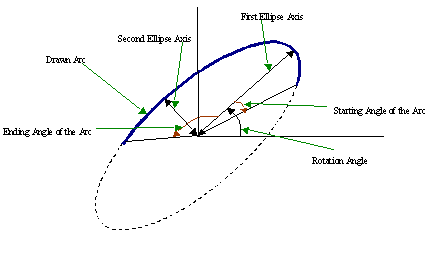
\includegraphics[width=0.5\textwidth]{pics/ellipse.png}

\cvCppFunc{ellipse2Poly}
Approximates an elliptic arc with a polyline

\cvdefCpp{
void ellipse2Poly( Point center, Size axes, int angle,\par
                   int startAngle, int endAngle, int delta,\par
                   vector<Point>\& pts );\newline
}
\begin{description}
\cvarg{center}{Center of the arc}
\cvarg{axes}{Half-sizes of the arc. See \cvCppCross{ellipse}}
\cvarg{angle}{Rotation angle of the ellipse in degrees. See \cvCppCross{ellipse}}
\cvarg{startAngle}{Starting angle of the elliptic arc in degrees}
\cvarg{endAngle}{Ending angle of the elliptic arc in degrees}
\cvarg{delta}{Angle between the subsequent polyline vertices. It defines the approximation accuracy.}
\cvarg{pts}{The output vector of polyline vertices}
\end{description}

The function \texttt{ellipse2Poly} computes the vertices of a polyline that approximates the specified elliptic arc. It is used by \cvCppCross{ellipse}.

\cvCppFunc{fillConvexPoly}
Fills a convex polygon.

\cvdefCpp{
void fillConvexPoly(Mat\& img, const Point* pts, int npts,\par
                    const Scalar\& color, int lineType=8,\par
                    int shift=0);\newline
}
\begin{description}
\cvarg{img}{Image}
\cvarg{pts}{The polygon vertices}
\cvarg{npts}{The number of polygon vertices}
\cvarg{color}{Polygon color}
\cvarg{lineType}{Type of the polygon boundaries, see \cvCppCross{line} description}
\cvarg{shift}{The number of fractional bits in the vertex coordinates}
\end{description}

The function \texttt{fillConvexPoly} draws a filled convex polygon.
This function is much faster than the function \texttt{fillPoly}
and can fill not only convex polygons but any monotonic polygon without self-intersections,
i.e., a polygon whose contour intersects every horizontal line (scan
line) twice at the most (though, its top-most and/or the bottom edge could be horizontal).

\cvCppFunc{fillPoly}
Fills the area bounded by one or more polygons

\cvdefCpp{void fillPoly(Mat\& img, const Point** pts, \par
              const int* npts, int ncontours,\par
              const Scalar\& color, int lineType=8,\par
              int shift=0, Point offset=Point() );}
\begin{description}
\cvarg{img}{Image}
\cvarg{pts}{Array of polygons, each represented as an array of points}
\cvarg{npts}{The array of polygon vertex counters}
\cvarg{ncontours}{The number of contours that bind the filled region}
\cvarg{color}{Polygon color}
\cvarg{lineType}{Type of the polygon boundaries, see \cvCppCross{line} description}
\cvarg{shift}{The number of fractional bits in the vertex coordinates}
\end{description}

The function \texttt{fillPoly} fills an area bounded by several
polygonal contours. The function can fills complex areas, for example,
areas with holes, contours with self-intersections (some of thier parts), and so forth.

\cvCppFunc{getTextSize}
Calculates the width and height of a text string.

\cvdefCpp{Size getTextSize(const string\& text, int fontFace,\par
                 double fontScale, int thickness,\par
                 int* baseLine);\newline}
\begin{description}
\cvarg{text}{The input text string}
\cvarg{fontFace}{The font to use; see \cvCppCross{putText}}
\cvarg{fontScale}{The font scale; see \cvCppCross{putText}}
\cvarg{thickness}{The thickness of lines used to render the text; see \cvCppCross{putText}}
\cvarg{baseLine}{The output parameter - y-coordinate of the baseline relative to the bottom-most text point}
\end{description}

The function \texttt{getTextSize} calculates and returns size of the box that contain the specified text.
That is, the following code will render some text, the tight box surrounding it and the baseline:

\begin{lstlisting}
// Use "y" to show that the baseLine is about
string text = "Funny text inside the box";
int fontFace = FONT_HERSHEY_SCRIPT_SIMPLEX;
double fontScale = 2;
int thickness = 3;

Mat img(600, 800, CV_8UC3, Scalar::all(0));

int baseline=0;
Size textSize = getTextSize(text, fontFace,
                            fontScale, thickness, &baseline);
baseline += thickness;

// center the text
Point textOrg((img.cols - textSize.width)/2,
              (img.rows + textSize.height)/2);

// draw the box
rectangle(img, textOrg + Point(0, baseline),
          textOrg + Point(textSize.width, -textSize.height),
          Scalar(0,0,255));
// ... and the baseline first
line(img, textOrg + Point(0, thickness),
     textOrg + Point(textSize.width, thickness),
     Scalar(0, 0, 255));

// then put the text itself
putText(img, text, textOrg, fontFace, fontScale,
        Scalar::all(255), thickness, 8);
\end{lstlisting}
        
        
\cvCppFunc{line}
Draws a line segment connecting two points

\cvdefCpp{void line(Mat\& img, Point pt1, Point pt2, const Scalar\& color,\par
          int thickness=1, int lineType=8, int shift=0);\newline}
\begin{description}
\cvarg{img}{The image}
\cvarg{pt1}{First point of the line segment}
\cvarg{pt2}{Second point of the line segment}
\cvarg{color}{Line color}
\cvarg{thickness}{Line thickness}
\cvarg{lineType}{Type of the line:
  \begin{description}
  \cvarg{8}{(or omitted) 8-connected line.}
  \cvarg{4}{4-connected line.}
  \cvarg{CV\_AA}{antialiased line.}
  \end{description}}
\cvarg{shift}{Number of fractional bits in the point coordinates}
\end{description}

The function \texttt{line} draws the line segment between
\texttt{pt1} and \texttt{pt2} points in the image. The line is
clipped by the image boundaries. For non-antialiased lines
with integer coordinates the 8-connected or 4-connected Bresenham
algorithm is used. Thick lines are drawn with rounding endings.
Antialiased lines are drawn using Gaussian filtering. To specify
the line color, the user may use the macro
\texttt{CV\_RGB(r, g, b)}.


\cvclass{LineIterator}
Class for iterating pixels on a raster line

\begin{lstlisting}
class LineIterator
{
public:
    // creates iterators for the line connecting pt1 and pt2
    // the line will be clipped on the image boundaries
    // the line is 8-connected or 4-connected
    // If leftToRight=true, then the iteration is always done
    // from the left-most point to the right most,
    // not to depend on the ordering of pt1 and pt2 parameters
    LineIterator(const Mat& img, Point pt1, Point pt2,
                 int connectivity=8, bool leftToRight=false);newline
    // returns pointer to the current line pixel
    uchar* operator *();newline
    // move the iterator to the next pixel
    LineIterator& operator ++();newline
    LineIterator operator ++(int);newline

    // internal state of the iterator
    uchar* ptr;newline
    int err, count;newline
    int minusDelta, plusDelta;newline
    int minusStep, plusStep;newline
};
\end{lstlisting}

The class \texttt{LineIterator} is used to get each pixel of a raster line. It can be treated as versatile implementation of the Bresenham algorithm, where you can stop at each pixel and do some extra processing, for example, grab pixel values along the line, or draw a line with some effect (e.g. with XOR operation).

The number of pixels along the line is store in \texttt{LineIterator::count}.

\begin{lstlisting}
// grabs pixels along the line (pt1, pt2)
// from 8-bit 3-channel image to the buffer
LineIterator it(img, pt1, pt2, 8);
vector<Vec3b> buf(it.count);

for(int i = 0; i < it.count; i++, ++it)
    buf[i] = *(const Vec3b)*it;
\end{lstlisting}


\cvCppFunc{rectangle}
Draws a simple, thick, or filled up-right rectangle.

\cvdefCpp{void rectangle(Mat\& img, Point pt1, Point pt2,\par
               const Scalar\& color, int thickness=1,\par
               int lineType=8, int shift=0);}
\begin{description}
\cvarg{img}{Image}
\cvarg{pt1}{One of the rectangle's vertices}
\cvarg{pt2}{Opposite to \texttt{pt1} rectangle vertex}
\cvarg{color}{Rectangle color or brightness (grayscale image)}
\cvarg{thickness}{Thickness of lines that make up the rectangle. Negative values, e.g. \texttt{CV\_FILLED}, mean that the function has to draw a filled rectangle.}
\cvarg{lineType}{Type of the line, see \cvCppCross{line} description}
\cvarg{shift}{Number of fractional bits in the point coordinates}
\end{description}

The function \texttt{rectangle} draws a rectangle outline or a filled rectangle, which two opposite corners are \texttt{pt1} and \texttt{pt2}.
               

\cvCppFunc{polylines}
Draws several polygonal curves

\cvdefCpp{void polylines(Mat\& img, const Point** pts, const int* npts,\par
               int ncontours, bool isClosed, const Scalar\& color,\par
               int thickness=1, int lineType=8, int shift=0 );\newline}
\begin{description}
\cvarg{img}{The image}
\cvarg{pts}{Array of polygonal curves}
\cvarg{npts}{Array of polygon vertex counters}
\cvarg{ncontours}{The number of curves}
\cvarg{isClosed}{Indicates whether the drawn polylines are closed or not. If they are closed, the function draws the line from the last vertex of each curve to its first vertex}
\cvarg{color}{Polyline color}
\cvarg{thickness}{Thickness of the polyline edges}
\cvarg{lineType}{Type of the line segments, see \cvCppCross{line} description}
\cvarg{shift}{The number of fractional bits in the vertex coordinates}
\end{description}

The function \texttt{polylines} draws one or more polygonal curves.

\cvCppFunc{putText}
Draws a text string

\cvdefCpp{void putText( Mat\& img, const string\& text, Point org,\par
              int fontFace, double fontScale, Scalar color,\par
              int thickness=1, int lineType=8,\par
              bool bottomLeftOrigin=false );}
\begin{description}
\cvarg{img}{The image}
\cvarg{text}{The text string to be drawn}
\cvarg{org}{The bottom-left corner of the text string in the image}
\cvarg{fontFace}{The font type, one of \texttt{FONT\_HERSHEY\_SIMPLEX}, \texttt{FONT\_HERSHEY\_PLAIN},
 \texttt{FONT\_HERSHEY\_DUPLEX}, \texttt{FONT\_HERSHEY\_COMPLEX}, \texttt{FONT\_HERSHEY\_TRIPLEX},
 \texttt{FONT\_HERSHEY\_COMPLEX\_SMALL}, \texttt{FONT\_HERSHEY\_SCRIPT\_SIMPLEX} or \texttt{FONT\_HERSHEY\_SCRIPT\_COMPLEX},
   where each of the font id's can be combined with \texttt{FONT\_HERSHEY\_ITALIC} to get the slanted letters.}
\cvarg{fontScale}{The font scale factor that is multiplied by the font-specific base size}
\cvarg{color}{The text color}
\cvarg{thickness}{Thickness of the lines used to draw the text}
\cvarg{lineType}{The line type; see \texttt{line} for details}
\cvarg{bottomLeftOrigin}{When true, the image data origin is at the bottom-left corner, otherwise it's at the top-left corner}
\end{description}

The function \texttt{putText} renders the specified text string in the image.
Symbols that can not be rendered using the specified font are
replaced by question marks. See \cvCppCross{getTextSize} for a text rendering code example.

\fi
